
%% bare_conf.tex
%% V1.4b
%% 2015/08/26
%% by Michael Shell
%% See:
%% http://www.michaelshell.org/
%% for current contact information.
%%
%% This is a skeleton file demonstrating the use of IEEEtran.cls
%% (requires IEEEtran.cls version 1.8b or later) with an IEEE
%% conference paper.
%%
%% Support sites:
%% http://www.michaelshell.org/tex/ieeetran/
%% http://www.ctan.org/pkg/ieeetran
%% and
%% http://www.ieee.org/

%%*************************************************************************
%% Legal Notice:
%% This code is offered as-is without any warranty either expressed or
%% implied; without even the implied warranty of MERCHANTABILITY or
%% FITNESS FOR A PARTICULAR PURPOSE! 
%% User assumes all risk.
%% In no event shall the IEEE or any contributor to this code be liable for
%% any damages or losses, including, but not limited to, incidental,
%% consequential, or any other damages, resulting from the use or misuse
%% of any information contained here.
%%
%% All comments are the opinions of their respective authors and are not
%% necessarily endorsed by the IEEE.
%%
%% This work is distributed under the LaTeX Project Public License (LPPL)
%% ( http://www.latex-project.org/ ) version 1.3, and may be freely used,
%% distributed and modified. A copy of the LPPL, version 1.3, is included
%% in the base LaTeX documentation of all distributions of LaTeX released
%% 2003/12/01 or later.
%% Retain all contribution notices and credits.
%% ** Modified files should be clearly indicated as such, including  **
%% ** renaming them and changing author support contact information. **
%%*************************************************************************


% *** Authors should verify (and, if needed, correct) their LaTeX system  ***
% *** with the testflow diagnostic prior to trusting their LaTeX platform ***
% *** with production work. The IEEE's font choices and paper sizes can   ***
% *** trigger bugs that do not appear when using other class files.       ***                          ***
% The testflow support page is at:
% http://www.michaelshell.org/tex/testflow/



\documentclass[conference]{IEEEtran}
% Some Computer Society conferences also require the compsoc mode option,
% but others use the standard conference format.
%
% If IEEEtran.cls has not been installed into the LaTeX system files,
% manually specify the path to it like:
% \documentclass[conference]{../sty/IEEEtran}





% Some very useful LaTeX packages include:
% (uncomment the ones you want to load)


% *** MISC UTILITY PACKAGES ***
%
%\usepackage{ifpdf}
% Heiko Oberdiek's ifpdf.sty is very useful if you need conditional
% compilation based on whether the output is pdf or dvi.
% usage:
% \ifpdf
%   % pdf code
% \else
%   % dvi code
% \fi
% The latest version of ifpdf.sty can be obtained from:
% http://www.ctan.org/pkg/ifpdf
% Also, note that IEEEtran.cls V1.7 and later provides a builtin
% \ifCLASSINFOpdf conditional that works the same way.
% When switching from latex to pdflatex and vice-versa, the compiler may
% have to be run twice to clear warning/error messages.

\usepackage{booktabs} % for fancy tables
\usepackage{siunitx} % for formatted table columns
\newcolumntype{L}[1]{>{\raggedright\let\newline\\\arraybackslash\hspace{0pt}}m{#1}}
\newcolumntype{C}[1]{>{\centering\let\newline\\\arraybackslash\hspace{0pt}}m{#1}}
\newcolumntype{R}[1]{>{\raggedleft\let\newline\\\arraybackslash\hspace{0pt}}m{#1}}

% bibiliography
\usepackage[backend=biber,style=ieee, % bibliography style may be changed
sorting=none, % sorting=nyt % sorts by author, year, title
autocite=inline, sortcites=true, labelnumber=true, % for compressed cites
dashed=false, % show repeated authors (i.e. don't blank out names)
]{biblatex}
% Note that full references are used.
\addbibresource{../Thesis/template/biliography.bib}
%\nocite{*} % include non referenced citations



% *** CITATION PACKAGES ***
%
%\usepackage{cite}
% cite.sty was written by Donald Arseneau
% V1.6 and later of IEEEtran pre-defines the format of the cite.sty package
% \cite{} output to follow that of the IEEE. Loading the cite package will
% result in citation numbers being automatically sorted and properly
% "compressed/ranged". e.g., [1], [9], [2], [7], [5], [6] without using
% cite.sty will become [1], [2], [5]--[7], [9] using cite.sty. cite.sty's
% \cite will automatically add leading space, if needed. Use cite.sty's
% noadjust option (cite.sty V3.8 and later) if you want to turn this off
% such as if a citation ever needs to be enclosed in parenthesis.
% cite.sty is already installed on most LaTeX systems. Be sure and use
% version 5.0 (2009-03-20) and later if using hyperref.sty.
% The latest version can be obtained at:
% http://www.ctan.org/pkg/cite
% The documentation is contained in the cite.sty file itself.






% *** GRAPHICS RELATED PACKAGES ***
%
\usepackage{graphicx}
\ifCLASSINFOpdf
  %\usepackage[pdftex]{graphicx}
  % declare the path(s) where your graphic files are
  % \graphicspath{{../pdf/}{../jpeg/}}
  % and their extensions so you won't have to specify these with
  % every instance of \includegraphics
  % \DeclareGraphicsExtensions{.pdf,.jpeg,.png}
\else
  % or other class option (dvipsone, dvipdf, if not using dvips). graphicx
  % will default to the driver specified in the system graphics.cfg if no
  % driver is specified.
  % \usepackage[dvips]{graphicx}
  % declare the path(s) where your graphic files are
  % \graphicspath{{../eps/}}
  % and their extensions so you won't have to specify these with
  % every instance of \includegraphics
  % \DeclareGraphicsExtensions{.eps}
\fi
% graphicx was written by David Carlisle and Sebastian Rahtz. It is
% required if you want graphics, photos, etc. graphicx.sty is already
% installed on most LaTeX systems. The latest version and documentation
% can be obtained at: 
% http://www.ctan.org/pkg/graphicx
% Another good source of documentation is "Using Imported Graphics in
% LaTeX2e" by Keith Reckdahl which can be found at:
% http://www.ctan.org/pkg/epslatex
%
% latex, and pdflatex in dvi mode, support graphics in encapsulated
% postscript (.eps) format. pdflatex in pdf mode supports graphics
% in .pdf, .jpeg, .png and .mps (metapost) formats. Users should ensure
% that all non-photo figures use a vector format (.eps, .pdf, .mps) and
% not a bitmapped formats (.jpeg, .png). The IEEE frowns on bitmapped formats
% which can result in "jaggedy"/blurry rendering of lines and letters as
% well as large increases in file sizes.
%
% You can find documentation about the pdfTeX application at:
% http://www.tug.org/applications/pdftex





% *** MATH PACKAGES ***
%
\usepackage{commath} % for abs
\usepackage{amsmath}

% A popular package from the American Mathematical Society that provides
% many useful and powerful commands for dealing with mathematics.
%
% Note that the amsmath package sets \interdisplaylinepenalty to 10000
% thus preventing page breaks from occurring within multiline equations. Use:
%\interdisplaylinepenalty=2500
% after loading amsmath to restore such page breaks as IEEEtran.cls normally
% does. amsmath.sty is already installed on most LaTeX systems. The latest
% version and documentation can be obtained at:
% http://www.ctan.org/pkg/amsmath





% *** SPECIALIZED LIST PACKAGES ***
%
%\usepackage{algorithmic}
% algorithmic.sty was written by Peter Williams and Rogerio Brito.
% This package provides an algorithmic environment fo describing algorithms.
% You can use the algorithmic environment in-text or within a figure
% environment to provide for a floating algorithm. Do NOT use the algorithm
% floating environment provided by algorithm.sty (by the same authors) or
% algorithm2e.sty (by Christophe Fiorio) as the IEEE does not use dedicated
% algorithm float types and packages that provide these will not provide
% correct IEEE style captions. The latest version and documentation of
% algorithmic.sty can be obtained at:
% http://www.ctan.org/pkg/algorithms
% Also of interest may be the (relatively newer and more customizable)
% algorithmicx.sty package by Szasz Janos:
% http://www.ctan.org/pkg/algorithmicx




% *** ALIGNMENT PACKAGES ***
%
%\usepackage{array}
% Frank Mittelbach's and David Carlisle's array.sty patches and improves
% the standard LaTeX2e array and tabular environments to provide better
% appearance and additional user controls. As the default LaTeX2e table
% generation code is lacking to the point of almost being broken with
% respect to the quality of the end results, all users are strongly
% advised to use an enhanced (at the very least that provided by array.sty)
% set of table tools. array.sty is already installed on most systems. The
% latest version and documentation can be obtained at:
% http://www.ctan.org/pkg/array


% IEEEtran contains the IEEEeqnarray family of commands that can be used to
% generate multiline equations as well as matrices, tables, etc., of high
% quality.




% *** SUBFIGURE PACKAGES ***
%\ifCLASSOPTIONcompsoc
%  \usepackage[caption=false,font=normalsize,labelfont=sf,textfont=sf]{subfig}
%\else
%  \usepackage[caption=false,font=footnotesize]{subfig}
%\fi
% subfig.sty, written by Steven Douglas Cochran, is the modern replacement
% for subfigure.sty, the latter of which is no longer maintained and is
% incompatible with some LaTeX packages including fixltx2e. However,
% subfig.sty requires and automatically loads Axel Sommerfeldt's caption.sty
% which will override IEEEtran.cls' handling of captions and this will result
% in non-IEEE style figure/table captions. To prevent this problem, be sure
% and invoke subfig.sty's "caption=false" package option (available since
% subfig.sty version 1.3, 2005/06/28) as this is will preserve IEEEtran.cls
% handling of captions.
% Note that the Computer Society format requires a larger sans serif font
% than the serif footnote size font used in traditional IEEE formatting
% and thus the need to invoke different subfig.sty package options depending
% on whether compsoc mode has been enabled.
%
% The latest version and documentation of subfig.sty can be obtained at:
% http://www.ctan.org/pkg/subfig




% *** FLOAT PACKAGES ***
%
%\usepackage{fixltx2e}
% fixltx2e, the successor to the earlier fix2col.sty, was written by
% Frank Mittelbach and David Carlisle. This package corrects a few problems
% in the LaTeX2e kernel, the most notable of which is that in current
% LaTeX2e releases, the ordering of single and double column floats is not
% guaranteed to be preserved. Thus, an unpatched LaTeX2e can allow a
% single column figure to be placed prior to an earlier double column
% figure.
% Be aware that LaTeX2e kernels dated 2015 and later have fixltx2e.sty's
% corrections already built into the system in which case a warning will
% be issued if an attempt is made to load fixltx2e.sty as it is no longer
% needed.
% The latest version and documentation can be found at:
% http://www.ctan.org/pkg/fixltx2e


%\usepackage{stfloats}
% stfloats.sty was written by Sigitas Tolusis. This package gives LaTeX2e
% the ability to do double column floats at the bottom of the page as well
% as the top. (e.g., "\begin{figure*}[!b]" is not normally possible in
% LaTeX2e). It also provides a command:
%\fnbelowfloat
% to enable the placement of footnotes below bottom floats (the standard
% LaTeX2e kernel puts them above bottom floats). This is an invasive package
% which rewrites many portions of the LaTeX2e float routines. It may not work
% with other packages that modify the LaTeX2e float routines. The latest
% version and documentation can be obtained at:
% http://www.ctan.org/pkg/stfloats
% Do not use the stfloats baselinefloat ability as the IEEE does not allow
% \baselineskip to stretch. Authors submitting work to the IEEE should note
% that the IEEE rarely uses double column equations and that authors should try
% to avoid such use. Do not be tempted to use the cuted.sty or midfloat.sty
% packages (also by Sigitas Tolusis) as the IEEE does not format its papers in
% such ways.
% Do not attempt to use stfloats with fixltx2e as they are incompatible.
% Instead, use Morten Hogholm'a dblfloatfix which combines the features
% of both fixltx2e and stfloats:
%
% \usepackage{dblfloatfix}
% The latest version can be found at:
% http://www.ctan.org/pkg/dblfloatfix




% *** PDF, URL AND HYPERLINK PACKAGES ***
%
%\usepackage{url}
% url.sty was written by Donald Arseneau. It provides better support for
% handling and breaking URLs. url.sty is already installed on most LaTeX
% systems. The latest version and documentation can be obtained at:
% http://www.ctan.org/pkg/url
% Basically, \url{my_url_here}.
\usepackage[hidelinks]{hyperref}




% *** Do not adjust lengths that control margins, column widths, etc. ***
% *** Do not use packages that alter fonts (such as pslatex).         ***
% There should be no need to do such things with IEEEtran.cls V1.6 and later.
% (Unless specifically asked to do so by the journal or conference you plan
% to submit to, of course. )


% correct bad hyphenation here
\hyphenation{op-tical net-works semi-conduc-tor}


\begin{document}
%
% paper title
% Titles are generally capitalized except for words such as a, an, and, as,
% at, but, by, for, in, nor, of, on, or, the, to and up, which are usually
% not capitalized unless they are the first or last word of the title.
% Linebreaks \\ can be used within to get better formatting as desired.
% Do not put math or special symbols in the title.
\title{Effect of Governor Deadbands on Valve Travel using Long-Term Dynamic Simulation}


% author names and affiliations
% use a multiple column layout for up to three different
% affiliations
\author{\IEEEauthorblockN{Thad Haines and Matt Donnelly}
\IEEEauthorblockA{School of Mines and Engineering\\
Montana Technological University\\
Butte, Montana 59701%
}
%\and
%\IEEEauthorblockN{Homer Simpson}
%\IEEEauthorblockA{Twentieth Century Fox\\
%Springfield, USA\\
%Email: homer@thesimpsons.com}
%\and
%\IEEEauthorblockN{James Kirk\\ and Montgomery Scott}
%\IEEEauthorblockA{Starfleet Academy\\
%San Francisco, California 96678--2391\\
%Telephone: (800) 555--1212\\
%Fax: (888) 555--1212}
}

% conference papers do not typically use \thanks and this command
% is locked out in conference mode. If really needed, such as for
% the acknowledgment of grants, issue a \IEEEoverridecommandlockouts
% after \documentclass

% for over three affiliations, or if they all won't fit within the width
% of the page, use this alternative format:
% 
%\author{\IEEEauthorblockN{Michael Shell\IEEEauthorrefmark{1},
%Homer Simpson\IEEEauthorrefmark{2},
%James Kirk\IEEEauthorrefmark{3}, 
%Montgomery Scott\IEEEauthorrefmark{3} and
%Eldon Tyrell\IEEEauthorrefmark{4}}
%\IEEEauthorblockA{\IEEEauthorrefmark{1}School of Electrical and Computer Engineering\\
%Georgia Institute of Technology,
%Atlanta, Georgia 30332--0250\\ Email: see http://www.michaelshell.org/contact.html}
%\IEEEauthorblockA{\IEEEauthorrefmark{2}Twentieth Century Fox, Springfield, USA\\
%Email: homer@thesimpsons.com}
%\IEEEauthorblockA{\IEEEauthorrefmark{3}Starfleet Academy, San Francisco, California 96678-2391\\
%Telephone: (800) 555--1212, Fax: (888) 555--1212}
%\IEEEauthorblockA{\IEEEauthorrefmark{4}Tyrell Inc., 123 Replicant Street, Los Angeles, California 90210--4321}}


% use for special paper notices
%\IEEEspecialpapernotice{(Invited Paper)}


% make the title area
\maketitle

% As a general rule, do not put math, special symbols or citations
% in the abstract
\begin{abstract}
Abstract goes here.
\end{abstract}

% no keywords
\begin{IEEEkeywords}
Governor deadbands, 
long-term dynamic simulation, 
time-sequenced power flow,
valve travel
\end{IEEEkeywords}

% For peer review papers, you can put extra information on the cover
% page as needed:
% \ifCLASSOPTIONpeerreview
% \begin{center} \bfseries EDICS Category: 3-BBND \end{center}
% \fi
%
% For peerreview papers, this IEEEtran command inserts a page break and
% creates the second title. It will be ignored for other modes.
\IEEEpeerreviewmaketitle

% Altered to use inputs
\section{Introduction}
Deadbands are commonly implemented in turbine speed governors to prevent a machine from responding to small frequency deviations that are ever present in electrical systems.
Industry usage of deadbands is widely known, however, it is often overlooked in power system simulation.
Incorporating governor deadbands into transient simulation models has been shown to generate results that better match measured power system events\cite{kou2016}.
Additionally, numerous long-term operational benefits have been attributed to the alteration of deadband behavior\cite{nercFRI2012}.
To better understand how deadbands may affect system behavior, a long-term simulation would seem suitable.
Long-term dynamic (LTD) simulation software focusing on governor dynamics was proposed in \cite{AGCCresap} and others, but has not been standardized nor fully developed.


This paper explores the impact of governor deadbands using a novel LTD simulation environment based on GE Energy's Positive Sequence Load Flow (PSLF) system models, dynamic data, and load flow solver. 
Valve travel as a metric for comparing the impact of various deadband scenarios is proposed. 
Section II describes the LTD simulation environment used to perform the studies. 
Section III discusses governor and deadband modeling within the simulation environment. 
In Section IV, the LTD simulation is validated against mature transient stability simulation. 
Finally, Section V presents some initial results demonstrating the viability of the proposed valve travel metric and Section VI offers conclusions.

\section{Long-Term Dynamic Simulation Technique}
Time-sequenced power flow (TSPF) is a method for LTD simulation proven to generate useful results\cite{DonnellyVoltageControl}.
The basic idea behind TSPF is to solve a power flow, calculate system dynamics of interest independent of the power-flow solver, `re-seed' the power flow with new values, and repeat.
%While this task is monotonous for humans, it is well suited for computers.
A Python based simulation software, Power System Long-Term Dynamic Simulator (PSLTDSim), has been developed to perform LTD simulations using TSPF.
PSLTDSim has the ability to calculate system frequency, perform governor dynamics, model automatic generation control (AGC), and insert step, ramp, and noise type perturbances into a power system.

%-------------------------------------------------------------------------------------
\subsection{Simulation Assumptions and Simplifications}
Due to the relatively large time steps of 1 second used with TSPF, numerous assumptions can be made.
Ideal exciters were assumed as modern exicters are typically fast enough to maintain reference voltage under stable conditions.
Intermachine oscillations were ignored since the time resolution used is not fine enough to capture these phenomena.

Simplifications of CTSS models are used in PSLTDSim.
The only parameters required to model a generator are the machine's rated MW, MVA base, and inertia.
Additionally, a deadband modified tgov1 governor model, shown in Fig. \ref{fig: tgov1BlockDiagram},  was created to model turbine speed governors.

\begin{figure}[!ht]
	\centering
	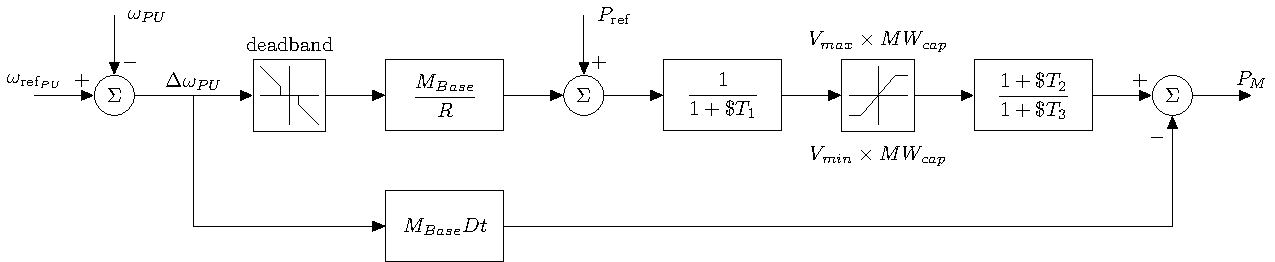
\includegraphics[width=\linewidth]{figures/tgov1DB}
	\caption{Block diagram of modified tgov1 model.}
	\label{fig: tgov1BlockDiagram}
\end{figure}

%-------------------------------------------------------------------------------------
\subsection{Modeling the System-Wide Frequency Response}
Instead of frequency being calculated for every bus, a combined swing equation is used to model only one system frequency.
As shown in (\ref{eq: CombinedSwingEq}), $\dot{\omega}_{sys}$ is calculated using accelerating power from the entire system, $P_{acc PU, sys}$, and total system inertia $H_{PU, sys}$.
An aggregate system frequency can then be found by integrating $\dot{\omega}_{sys}$.

\begin{align}
\dot{\omega}_{sys} = \dfrac{1}{2H_{PU, sys} } \left( \dfrac{P_{acc PU, sys} }{\omega_{sys}} - D_{sys}\Delta\omega_{sys}  \right) \label{eq: CombinedSwingEq}
\end{align} 

%-------------------------------------------------------------------------------------
\subsection{Distribution of Accelerating Power}
In a system with $N$ generators, total system accelerating power is calculated by
\begin{align}
P_{acc, sys} = \sum_{i=1}^{N} P_{m,i}  - \sum_{i=1}^{N} P_{e,i} \label{eq:Pacc} 
\end{align}
\noindent where $P_{m,i}$ is mechanical power and $P_{e,i}$ is electrical power of generator $i$.

System accelerating power is distributed to all generators in the system according to machine inertia as
\begin{align}
P_{e, i} = P_{e, i}  - P_{acc, sys}\left( \dfrac{H_i}{H_{sys}}\right) \label{eq:distPacc}
\end{align}
where $H$ has units of $MW\cdot s$.

The new value for $P_{e, i}$ is used in the next power flow solution for each generator.
%Once all accelerating power is distributed, the new value for each generators power output is used as initial conditions to solve a power flow. 
If the difference between expected and resulting power supplied by the slack generator is larger than a set slack tolerance, the difference is redistributed according to (\ref{eq:distPacc}) until the resulting difference is below the slack tolerance, or a maximum number of iterations take place\cite{Stajcar}.

\section{Implementation of Deadbands}
FERC Order 842 specifies governor droop of 5\% deadbands of a maximum 36 mHz\cite{ferc2018}.
Several types of deadbands are currently used in practice as practical implementation is left to generator operators.

\subsection{Types of Deadbands}
Fig. \ref{fig: deadbandType} presents implementations of deadbands that meet FERC specifications.
If a governor has no deadband, a change in output power is requested for any frequency deviation.
A step deadband ignores any frequency smaller than the setpoint $\pm db_1$ and then steps to meet the set droop curve.
A no-step deadband pushes the original droop curve away from the nominal frequency allowing for the droop curve to cross zero at $\pm db_2$ but never return to the step or no deadband droop curve.
A non-linear deadband is introduced that linearly increases from $\pm \alpha$ to $\pm \beta$, after which it follows the original droop curve.

\begin{figure}[!ht]
	\centering
	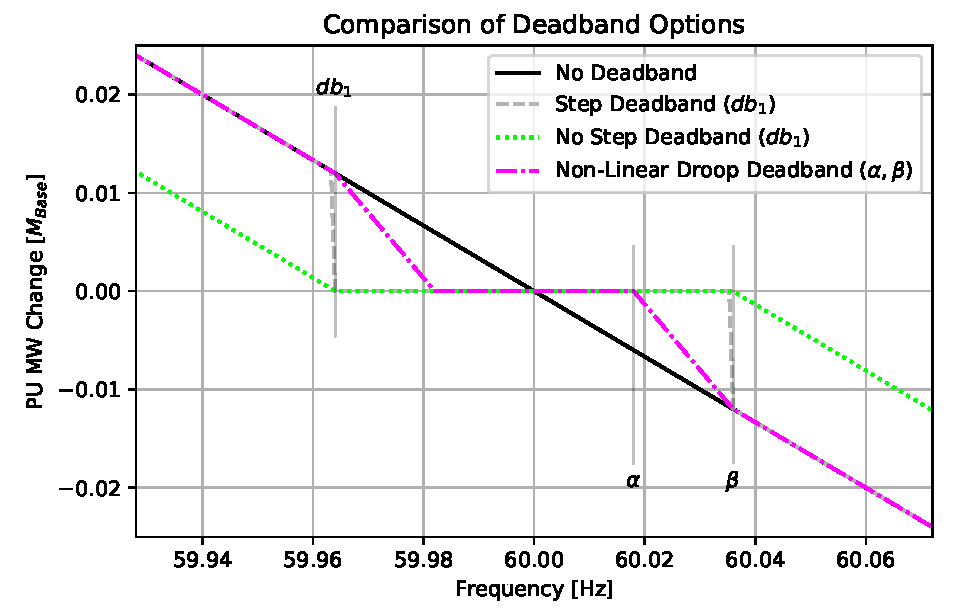
\includegraphics[width=\linewidth]{figures/dbAction3}
	\caption{Different types of deadbands.}
	\label{fig: deadbandType}
\end{figure}
\section{Simulation Validation}
To validate the chosen simulation approach, identical system perterbations were simulated in both the PSLF Dynamic Subsystem (PSDS), a classical transient stability simulation environment, and PSLTDSim.
%The output data was then compared in MATLAB.
Frequency comparisons were used to validate the single system frequency assumption calculated by PSLTDSim. Comparisons of the mechanical power of governed generators were used to validate governor action.

Comparison of frequency data from PSDS to LTD was simplified by calculating a single weighted PSDS frequency $f_w$ based on generator inertia. 
In a system with $N$ generators
\begin{align}
f_{w} &= \sum_{i=1}^{N} f_i \dfrac{H_{PU, i} M_{base, i} }{H_{sys}}  \label{eq: f_weighted}\\
\text{where } H_{sys} &= \sum_{i=1}^{N} H_{PU, i} M_{base, i}.  \label{eq: Hsys}
\end{align}
% This explanation may be unnecessary for IEEE... removed for space
%Due to the different time steps, when calculating the difference between PSDS and LTD, multiple PSDS values have the same held LTD value subtracted from them. 
%For instance, any PSDS($t = 3.x$) value would have the LTD($t = 3$) value subtracted from it for comparison.

% Something about an individual difference not mattering as much as the general difference, therfore all ltd psds comparisons are plotted as a single color.

%-------------------------------------------------------------------------------------
\subsection{The MiniWECC System}

The power system used for validation and valve travel experiments, the `miniWECC' shown in Fig. \ref{fig: miniWECC}, is a 120 bus 34 generator system created in PSLF.
The governored machines in the miniWECC were modeled with the tgov1 governor, which enabled easier validation.
Further details about the creation and use of the miniWECC may be found in \cite{trudnowski2012, sandia2015, RJminiWECC}.

\begin{figure}[!ht]
	\centering
	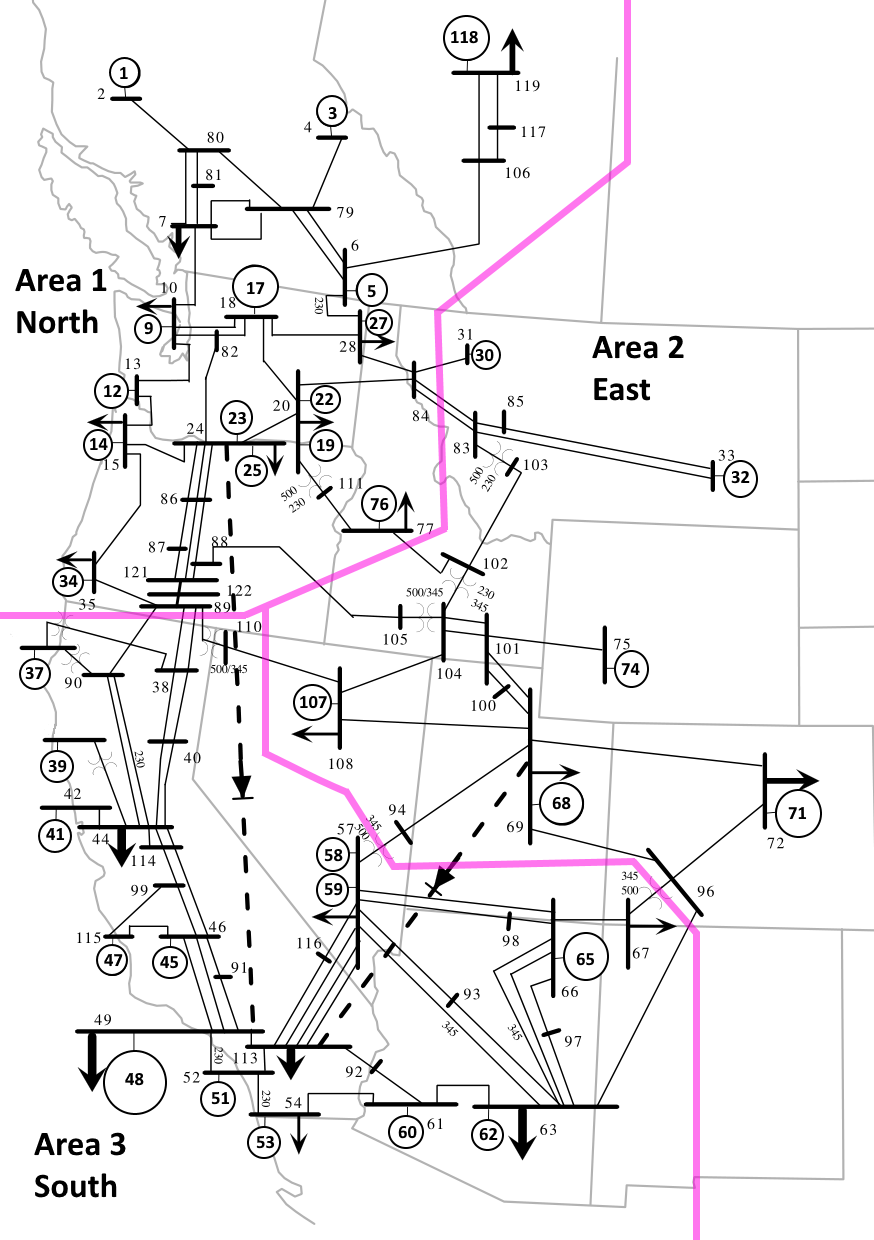
\includegraphics[width=.65\linewidth]{figures/miniWECC_split03}
	\caption{MiniWECC system adapted from \cite{RJminiWECC}.}
	\label{fig: miniWECC}
\end{figure}

%`````````````````````````````````````````````````````````````````````````````````````
\subsubsection{Load Step Results}
A 400 MW load step at $t$ = 2 seconds was used for validating the performance of the PSLTDSim.
As shown in Fig. \ref{fig: stepFcomp}, all individual PSDS frequencies begin to oscillate after the perturbance while the weighted PSDS frequency appears to follow the general center of oscillation. The LTD system frequency is less oscillatory than the weighted frequency with only minor differences between the two. Fig. \ref{fig: rampFdif} quantifies these frequency differences.

\begin{figure}[!t]
	\centering
	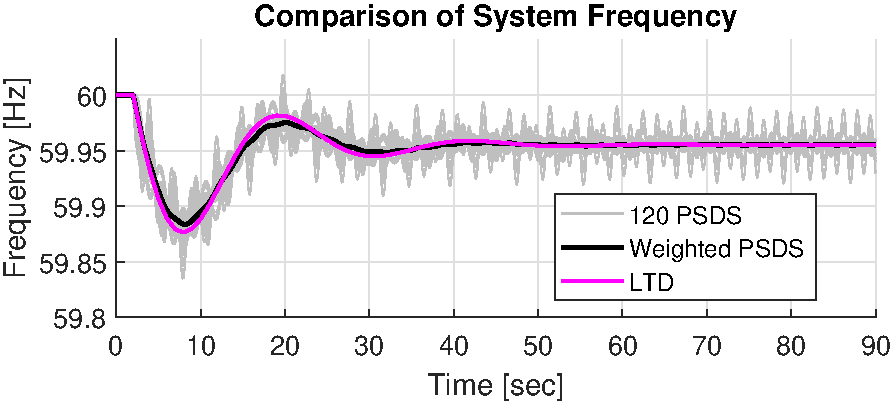
\includegraphics[width=\linewidth]{figures/miniWECC3ALTDstepF3}
	\caption{Comparison of frequency during load step.}
	\label{fig: stepFcomp}
\end{figure}

\begin{figure}[!t]
	\centering
	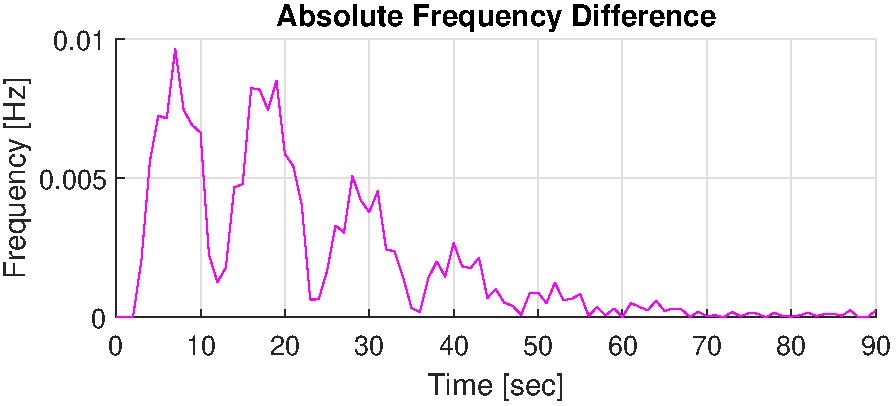
\includegraphics[width=\linewidth]{figures/miniWECC3ALTDstepRelF}
	\caption{Absolute difference of weighted frequency during load step.}
	\label{fig: stepFdif}
\end{figure}

When comparing mechanical power in Fig. \ref{fig: stepPmdif}, large MW differences can be seen, however, the percent difference data in Fig. \ref{fig: stepPmPercentdif} shows results less than 5\% max difference, and an average percent difference of less than $\approx$0.5\%.

\begin{figure}[!ht]
	\centering
	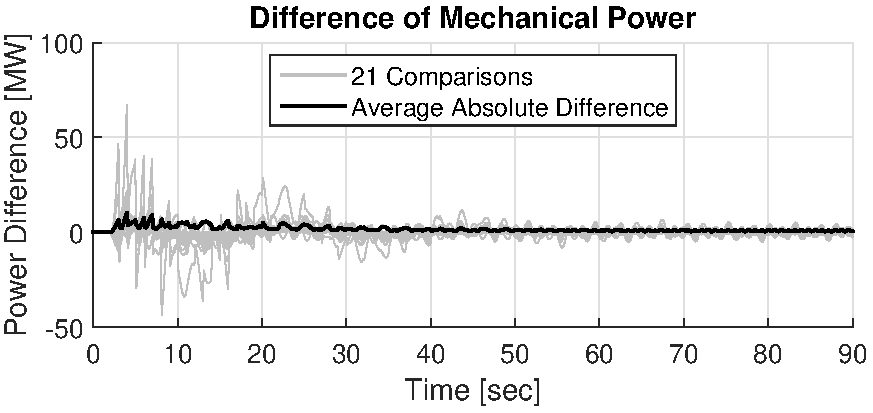
\includegraphics[width=\linewidth]{figures/miniWECC3ALTDstepPm2}
	\caption{Difference of mechanical power during load step.}
	\label{fig: stepPmdif}
\end{figure}

\begin{figure}[!ht]
	\centering
	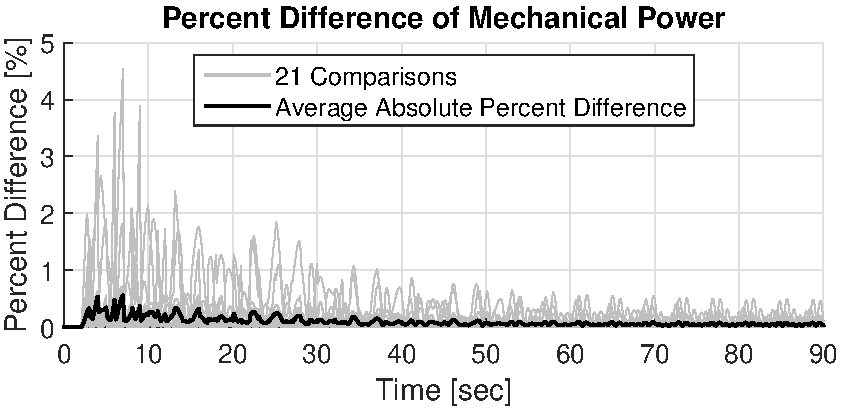
\includegraphics[width=\linewidth]{figures/miniWECC3ALTDstepPm3}
	\caption{Percent difference of mechanical power during load step.}
	\label{fig: stepPmPercentdif}
\end{figure}


%`````````````````````````````````````````````````````````````````````````````````````
\subsubsection{Load Ramp Results}
A second set of validation results, using a 40 second 400 MW load ramp, were also generated. Figs. \ref{fig: rampFcomp}-\ref{fig: rampFdif} show frequency of LTD being within 1.5 mHz of PSDS.
Fig. \ref{fig: rampPmdif} shows mechanical power differences of less than $\pm$10 MW or, as Fig. \ref{fig: rampPmPercentdif} shows, 1\% difference max.
%*** Ramp results are included for now, but may be take up too much space... They do function as a `better' validation...

\begin{figure}[!ht]
	\centering
	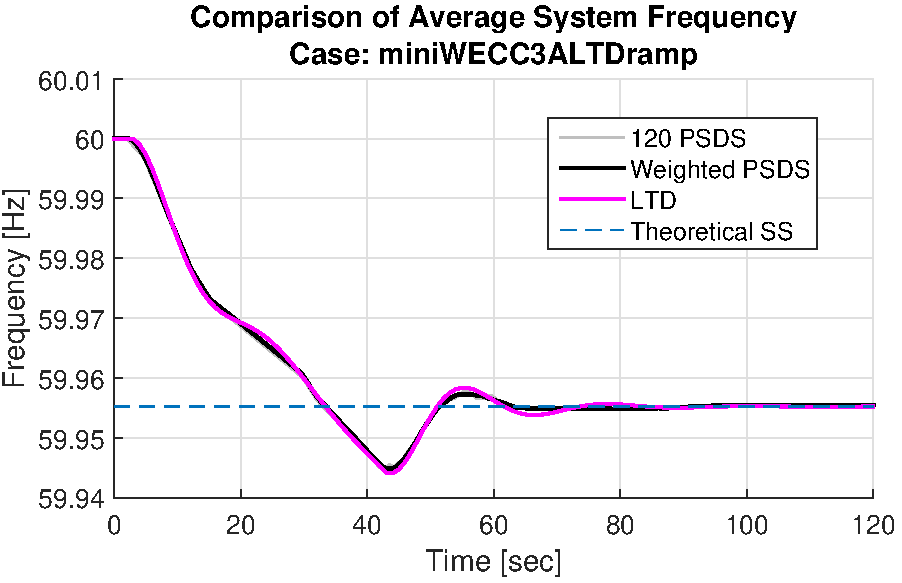
\includegraphics[width=\linewidth]{figures/miniWECC3ALTDrampF3}
	\caption{Comparison of frequency during load ramp.}
	\label{fig: rampFcomp}
\end{figure}

\begin{figure}[!ht]
	\centering
	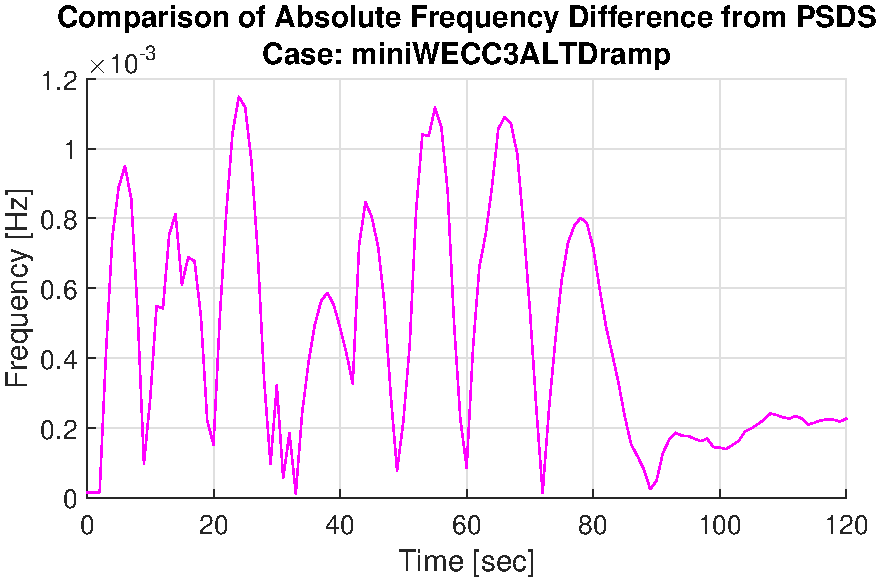
\includegraphics[width=\linewidth]{figures/miniWECC3ALTDrampRelF}
	\caption{Absolute difference of weighted frequency during load ramp.}
	\label{fig: rampFdif}
\end{figure}

\begin{figure}[!ht]
	\centering
	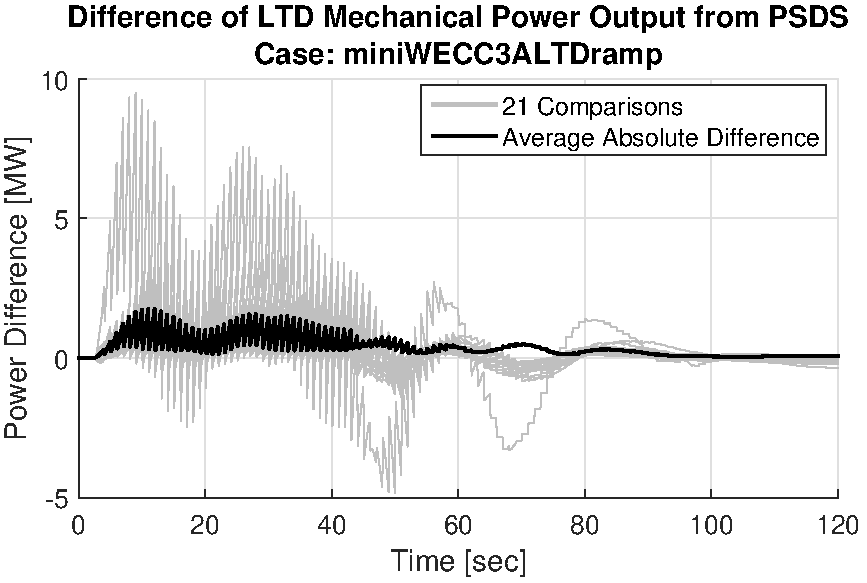
\includegraphics[width=\linewidth]{figures/miniWECC3ALTDrampPm2}
	\caption{Difference of mechanical power during load ramp.}
	\label{fig: rampPmdif}
\end{figure}

\begin{figure}[!ht]
	\centering
	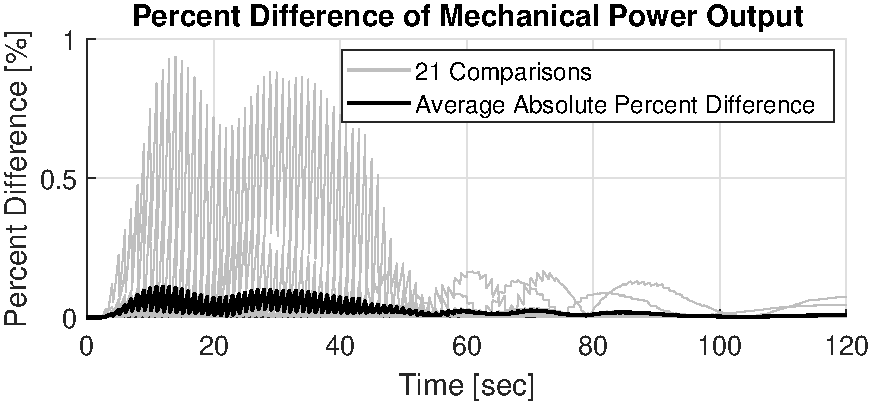
\includegraphics[width=\linewidth]{figures/miniWECC3ALTDrampPm3}
	\caption{Percent difference of mechanical power during load ramp.}
	\label{fig: rampPmPercentdif}
\end{figure}
%-------------------------------------------------------------------------------------
\subsection{Validation Summary}
The validation results show that PSLTDSim accurately captures long term power system dyanmics. The step test results show that PSLTDSim cannot replace classical transient stability simultion for the study of large, short-duration transient events, however repeated small perturbances are modeled with acceptable deviation from transient simulation methods.
\section{Case Study}
Explanation of simulations to do...

30 minutes of noise with various deadbands and resulting valve travel.
Cases of interest:
No deadband, step deadband, no-step deadband, nl-droop deadband.

Universal acceptance sim:
At least 1 area with a step deadband, others with linear or no deadband.
Should show unequal distribution of valve travel.

\subsection{System Modifications}
The miniWECC system was modified to include three areas for AGC simulation.
PSLTDSim was used to set all area governor deadbands to 5\%.
Governors were removed from some units so that only $\approx$20\% of generation capacity in each area has governor control.
A generic AGC routine that filters area control error (ACE) through a proportional-intergal (PI)  controller was added to each area.
AGC messages are sent select generation units with governors representing $\approx$9\% of total generation capacity every 15 seconds.

\subsection{Simulation Results}
To verify desirable AGC control operation, a simple 1500 MW generation loss event was simulated...

...
Noise test frequency plots and valve travel movement, table of results
\section{Conclusion}
Maybe having deadbands is a bad move - extra work caused by procrastination.
Though everyone needs to be on board, else maybe they can get a free ride.

% An example of a floating figure using the graphicx package.
% Note that \label must occur AFTER (or within) \caption.
% For figures, \caption should occur after the \includegraphics.
% Note that IEEEtran v1.7 and later has special internal code that
% is designed to preserve the operation of \label within \caption
% even when the captionsoff option is in effect. However, because
% of issues like this, it may be the safest practice to put all your
% \label just after \caption rather than within \caption{}.
%
% Reminder: the "draftcls" or "draftclsnofoot", not "draft", class
% option should be used if it is desired that the figures are to be
% displayed while in draft mode.
%
%\begin{figure}[!t]
%\centering
%\includegraphics[width=2.5in]{myfigure}
% where an .eps filename suffix will be assumed under latex, 
% and a .pdf suffix will be assumed for pdflatex; or what has been declared
% via \DeclareGraphicsExtensions.
%\caption{Simulation results for the network.}
%\label{fig_sim}
%\end{figure}

% Note that the IEEE typically puts floats only at the top, even when this
% results in a large percentage of a column being occupied by floats.


% An example of a double column floating figure using two subfigures.
% (The subfig.sty package must be loaded for this to work.)
% The subfigure \label commands are set within each subfloat command,
% and the \label for the overall figure must come after \caption.
% \hfil is used as a separator to get equal spacing.
% Watch out that the combined width of all the subfigures on a 
% line do not exceed the text width or a line break will occur.
%
%\begin{figure*}[!t]
%\centering
%\subfloat[Case I]{\includegraphics[width=2.5in]{box}%
%\label{fig_first_case}}
%\hfil
%\subfloat[Case II]{\includegraphics[width=2.5in]{box}%
%\label{fig_second_case}}
%\caption{Simulation results for the network.}
%\label{fig_sim}
%\end{figure*}
%
% Note that often IEEE papers with subfigures do not employ subfigure
% captions (using the optional argument to \subfloat[]), but instead will
% reference/describe all of them (a), (b), etc., within the main caption.
% Be aware that for subfig.sty to generate the (a), (b), etc., subfigure
% labels, the optional argument to \subfloat must be present. If a
% subcaption is not desired, just leave its contents blank,
% e.g., \subfloat[].


% An example of a floating table. Note that, for IEEE style tables, the
% \caption command should come BEFORE the table and, given that table
% captions serve much like titles, are usually capitalized except for words
% such as a, an, and, as, at, but, by, for, in, nor, of, on, or, the, to
% and up, which are usually not capitalized unless they are the first or
% last word of the caption. Table text will default to \footnotesize as
% the IEEE normally uses this smaller font for tables.
% The \label must come after \caption as always.
%
%\begin{table}[!t]
%% increase table row spacing, adjust to taste
%\renewcommand{\arraystretch}{1.3}
% if using array.sty, it might be a good idea to tweak the value of
% \extrarowheight as needed to properly center the text within the cells
%\caption{An Example of a Table}
%\label{table_example}
%\centering
%% Some packages, such as MDW tools, offer better commands for making tables
%% than the plain LaTeX2e tabular which is used here.
%\begin{tabular}{|c||c|}
%\hline
%One & Two\\
%\hline
%Three & Four\\
%\hline
%\end{tabular}
%\end{table}


% Note that the IEEE does not put floats in the very first column
% - or typically anywhere on the first page for that matter. Also,
% in-text middle ("here") positioning is typically not used, but it
% is allowed and encouraged for Computer Society conferences (but
% not Computer Society journals). Most IEEE journals/conferences use
% top floats exclusively. 
% Note that, LaTeX2e, unlike IEEE journals/conferences, places
% footnotes above bottom floats. This can be corrected via the
% \fnbelowfloat command of the stfloats package.


% conference papers do not normally have an appendix


% use section* for acknowledgment
\section*{Acknowledgment}
The authors would like to thank...


% trigger a \newpage just before the given reference
% number - used to balance the columns on the last page
% adjust value as needed - may need to be readjusted if
% the document is modified later
%\IEEEtriggeratref{8}
% The "triggered" command can be changed if desired:
%\IEEEtriggercmd{\enlargethispage{-5in}}

% references section

% can use a bibliography generated by BibTeX as a .bbl file
% BibTeX documentation can be easily obtained at:
% http://mirror.ctan.org/biblio/bibtex/contrib/doc/
% The IEEEtran BibTeX style support page is at:
% http://www.michaelshell.org/tex/ieeetran/bibtex/
%\bibliographystyle{IEEEtran}
% argument is your BibTeX string definitions and bibliography database(s)
%\bibliography{IEEEabrv,../bib/paper}
%
% <OR> manually copy in the resultant .bbl file
% set second argument of \begin to the number of references
% (used to reserve space for the reference number labels box)

% Not standard operation, but seems to work.
\printbibliography


%\begin{thebibliography}{1}
%\bibitem{IEEEhowto:kopka}
%H.~Kopka and P.~W. Daly, \emph{A Guide to \LaTeX}, 3rd~ed.\hskip 1em plus
%  0.5em minus 0.4em\relax Harlow, England: Addison-Wesley, 1999.
%\end{thebibliography}


% template forms - To be removed before final version
\pagebreak
\section{Non-Text Format Templates}
This section meant to provide template figures, tables, equations, and references that can be copied and pasted to other parts of the document in a simple manner.

Figures will behave as Fig. \ref{fig: test}. Note that the placement may seem random, but is chosen by \LaTeX\ automatically.
\begin{figure}[!ht]
\centering
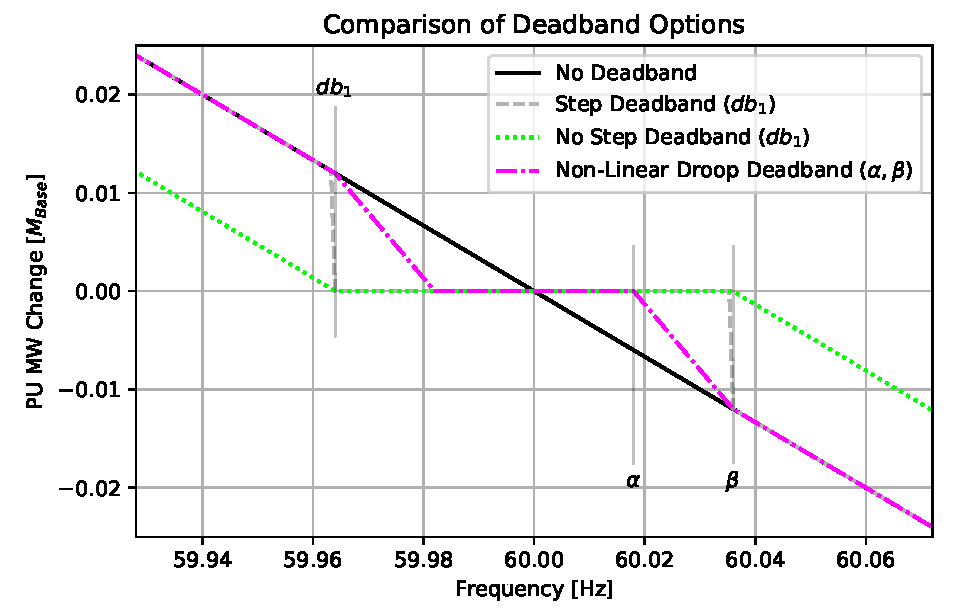
\includegraphics[width=\linewidth]{figures/dbAction3}
\caption{Testing of figure format.}
\label{fig: test}
\end{figure}


The default IEEE table example leaves something to be desired that is fulfilled by using the \verb|booktabs| package.
This is shown in Table \ref{tab: test2}.
% Testing of external table build for \input later
% Uses the IEEE table format guidelines
\begin{table}[!ht]
	\caption{Generic governor model parameters.}
	\label{tab: test2}
	\centering
	\begin{tabular}{@{} C{2cm} S[table-format=2.2] S[table-format=2.2] S[table-format=2.2] @{}} 	
		\toprule % @ signs to remove extra L R space
		\text{Parameter}	&	\text{Steam}	&	\text{Hydro}	&	\text{Gas}	\\		
		\midrule		
			Ts	&	0.04	&	0.40	&0.50\\
			Tc	&	0.20	&	45.00	&10.00\\
			T3	&	0.00	&	5.00	&4.00\\
			T4	&	1.50	&	-1.00	&0.00\\
			T5	&	5.00	&	0.50	&1.00\\
		\bottomrule
	\end{tabular}

\end{table}

Equations are entered as one may normally do in a \LaTeX\ situation and referenced as (\ref{eq: TestEq1}) and (\ref{eq: TestEq2}).
\begin{align}
f_{ss} &= f_{ref}+\Delta f = f_{ref} + \dfrac{\Delta P}{S_{Base}\beta}  \label{eq: TestEq1}\\
\beta &= \sum_{i=1}^{N} \dfrac{1}{R_i \frac{S_{Base}}{M_{Base, i}} } \label{eq: TestEq2}
\end{align}

References are only included if cited. For instance \cite{Kundur} or \cite{DonnellyVoltageControl} are randomly cited. Note that the sorting order is set to \verb|none|, which lists references in order cited.


% that's all folks
\end{document}